\documentclass[hyperref={pdfpagelabels=false}]{beamer}
\let\Tiny=\tiny
\mode<presentation>{
\usetheme{AnnArbor}
\usecolortheme{beaver}
\usefonttheme{serif}
}
\usepackage{default}
%\usepackage{ucs}
\usepackage[utf8]{inputenc}
\usepackage{gb4e}
\usepackage[T1]{fontenc}
\usepackage{ tipa }
\usepackage{qtree}
\usepackage{synttree}
%\usepackage{color}
\usepackage{tree-dvips}
\usepackage[absolute,overlay]{textpos}
%\usepackage{covington-beamer}
\usepackage{lmodern}
\usepackage{hyperref}
\usepackage{natbib}
\usepackage{graphicx}
\usepackage{eso-pic}
\usepackage{booktabs}
\usepackage{tikz}
%\usepackage{memoir}
%\usepackage{relsize}
%\newcommand{\subscript}[1]{\raisebox{-0.25em}{\smaller #1}}
%\logo{\includegraphics[height=1cm]{nclcbelogomono.eps}}
\setbeamertemplate{footline}[frame number] 
%gets rid of navigation symbols
\setbeamertemplate{navigation symbols}{}

\title{How I learned to stop worrying and love the leave}
\author{Joel C. Wallenberg\\\texttt{joel.wallenberg@ncl.ac.uk}}
\institute{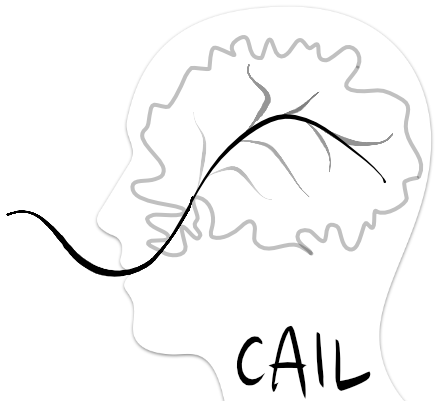
\includegraphics[scale = 0.2]{caillogo.png}}
%\date[]{14th May, 2019}

\begin{document}

\begin{frame}[plain]
\titlepage
\end{frame}

\begin{frame}{``Constraints on the Adaptiveness of Information in Language'' (CAIL)} 
	
	\begin{itemize}
		\item \small{\url{https://cail-project.github.io/}}
		\item Collaboration with Christine Cuskley and Rachael Bailes
		\item ESRC Secondary Data Analysis Initiative (SDAI), grant \#ES/T005955/1\\

	\end{itemize}


	\begin{center}
		\includegraphics[scale=0.2]{wallenbergetalheader.png}
	\end{center}
\rightline{\textsl{\citet{wallenbergetal2021}}}


\end{frame}


\begin{frame}
	\frametitle{Outline}
	\tableofcontents
\end{frame}


\section{Crash Course in Information Theory}

\begin{frame}{Crash course: Information theory and language} 
\begin{itemize}
	\item \textbf{Key Insight:} The amount of information a sender can theoretically communicate about an event is the uncertainty (``entropy'') the receiver has about the event beforehand, which may be reduced by a signal \citep{hartley1928, shannon1948}.
\end{itemize}
\begin{center}

	\includegraphics[scale=0.55]{../shannonSchematic.png} 


\end{center}



\end{frame}

\begin{frame}{Crash course: Information theory and language} 
	\begin{itemize}
		\item \textbf{Before the receiver gets any signal:} for a more uncertain event, more information could be communicated.
		\item \textbf{If the receiver gets a signal:} a low probability signal has given the receiver more information than a high probability one, regardless of how uncertain the event was. 
	\end{itemize}
	\begin{center}
			\includegraphics[scale=0.4]{bbcweather.jpg} 
	\end{center}
\end{frame}


\begin{frame}{Crash course: Information theory and language} 
	\begin{itemize}
		\item \citet{shannon1948}'s formula for information in an event with \textsl{n} discrete outcomes with probabilities p_1...p_n:
	\end{itemize}
	\begin{center}
		$$\sum_{1}^{n} p_i log_2 \frac{1}{p_i}$$
	\end{center}
	\begin{itemize}
		\item The $log_2 \frac{1}{p_i}$ part is the \textsl{information content} of an outcome.
		\item Lower probability signals provide more information when received, though they show up less often.
		\item The unit of information is a \textbf{``bit''}!
	\end{itemize}
	
\end{frame}


\begin{frame}{``Uniform Information Density'' in language} 
\begin{itemize}
	\item Any linguistic unit can be thought of as a signal to the overall content/function of an utterance.
	\item ``noise'' is any interference, including: noise, memory, other processing costs, etc.
	\item Speakers tend to spread information content across utterances as uniformly as possible \small{(\citealt{fenkfenk1980,aylettturk2004,levyjaeger2007}; Cuskley, Bailes \& Wallenberg, \textsl{Forthcoming})}.\nocite{cuskleyWallenberg2021}
\end{itemize}
\begin{exe}
	\ex How big is the family $[$(that) you cook for$]$?
\end{exe}

\begin{center}
	If \textsl{that} is deleted, more information is carried by \textsl{you}, so information is more dense.
\end{center}


\end{frame}



\begin{frame}{UID and noise resistance} 

\begin{center}
\includegraphics[scale=0.585]{../sentence1info.png} 
\end{center}

\end{frame}

\begin{frame}{UID and noise resistance} 

\begin{center}
	\includegraphics[scale=0.585]{../sentence2info.png} 
\end{center}

\end{frame}


\section{Study 1: OV-to-VO in English and Icelandic}

\begin{frame}{Study 1: OV-to-VO in English and Icelandic} 
	

	\textbf{Middle English:}
	\begin{exe}	
		\ex \label{julia}  \gll Mi feader \& Mi moder for-þi þt ich nule þe forsaken; habbe forsake me.\\
		My father and my mother because that I not+would you forsake have forsaken me\\
		\quad ``Because I would not forsake you, my father and mother have forsaken me''\\\vspace{2mm}
		\small{(\textsl{St. Juliana}, northern Herefordshire/southern Shropshire, date: c1225; ID CMJULIA-M1,106.172 from the \textsl{Penn Parsed Corpus of Middle English 2} \citep{ppcme24})}
	\end{exe}
	
\end{frame}

\begin{frame}{OV-to-VO in English and Icelandic} 
	
	\textbf{Historical Icelandic:}%This is not a list
	\begin{exe}\ex \label{ex:ntov}\begin{xlist}
			\ex {\gll \ldots og sannleikurinn mun yður frelsa \\
				\ldots and {the truth} will you free \\
				\quad ``\ldots and the truth will set you free.''  }\\\vspace{2mm}
			\small{(\textit{\small{Oddur Gottskálksson's New Testament}}, date: 1540; ID 1540.NTJOHN.REL-BIB, 204.662 from \textsl{Icelandic Parsed Historical Corpus} \citep{icepahc09})}\\\vspace{5mm}
			%1540.NTJOHN.REL-BIB,204.662
			\ex {\gll \ldots en eg skal sjá yður aftur. \\
				but I shall see you-\sc{pl} again\\
				\quad ``\ldots but I shall see you again'' \\\vspace{2mm}
				\small{(\textit{Oddur Gottskálksson's New Testament}, date: 1540; ID 1540.NTJOHN.REL-BIB, 223.1305 from IcePaHC)}
				% 1540.NTJOHN.REL-BIB,223.1305   
			}
		\end{xlist}
	\end{exe}
	

	
\end{frame}

\begin{frame}{OV-to-VO in English and Icelandic} 
	

	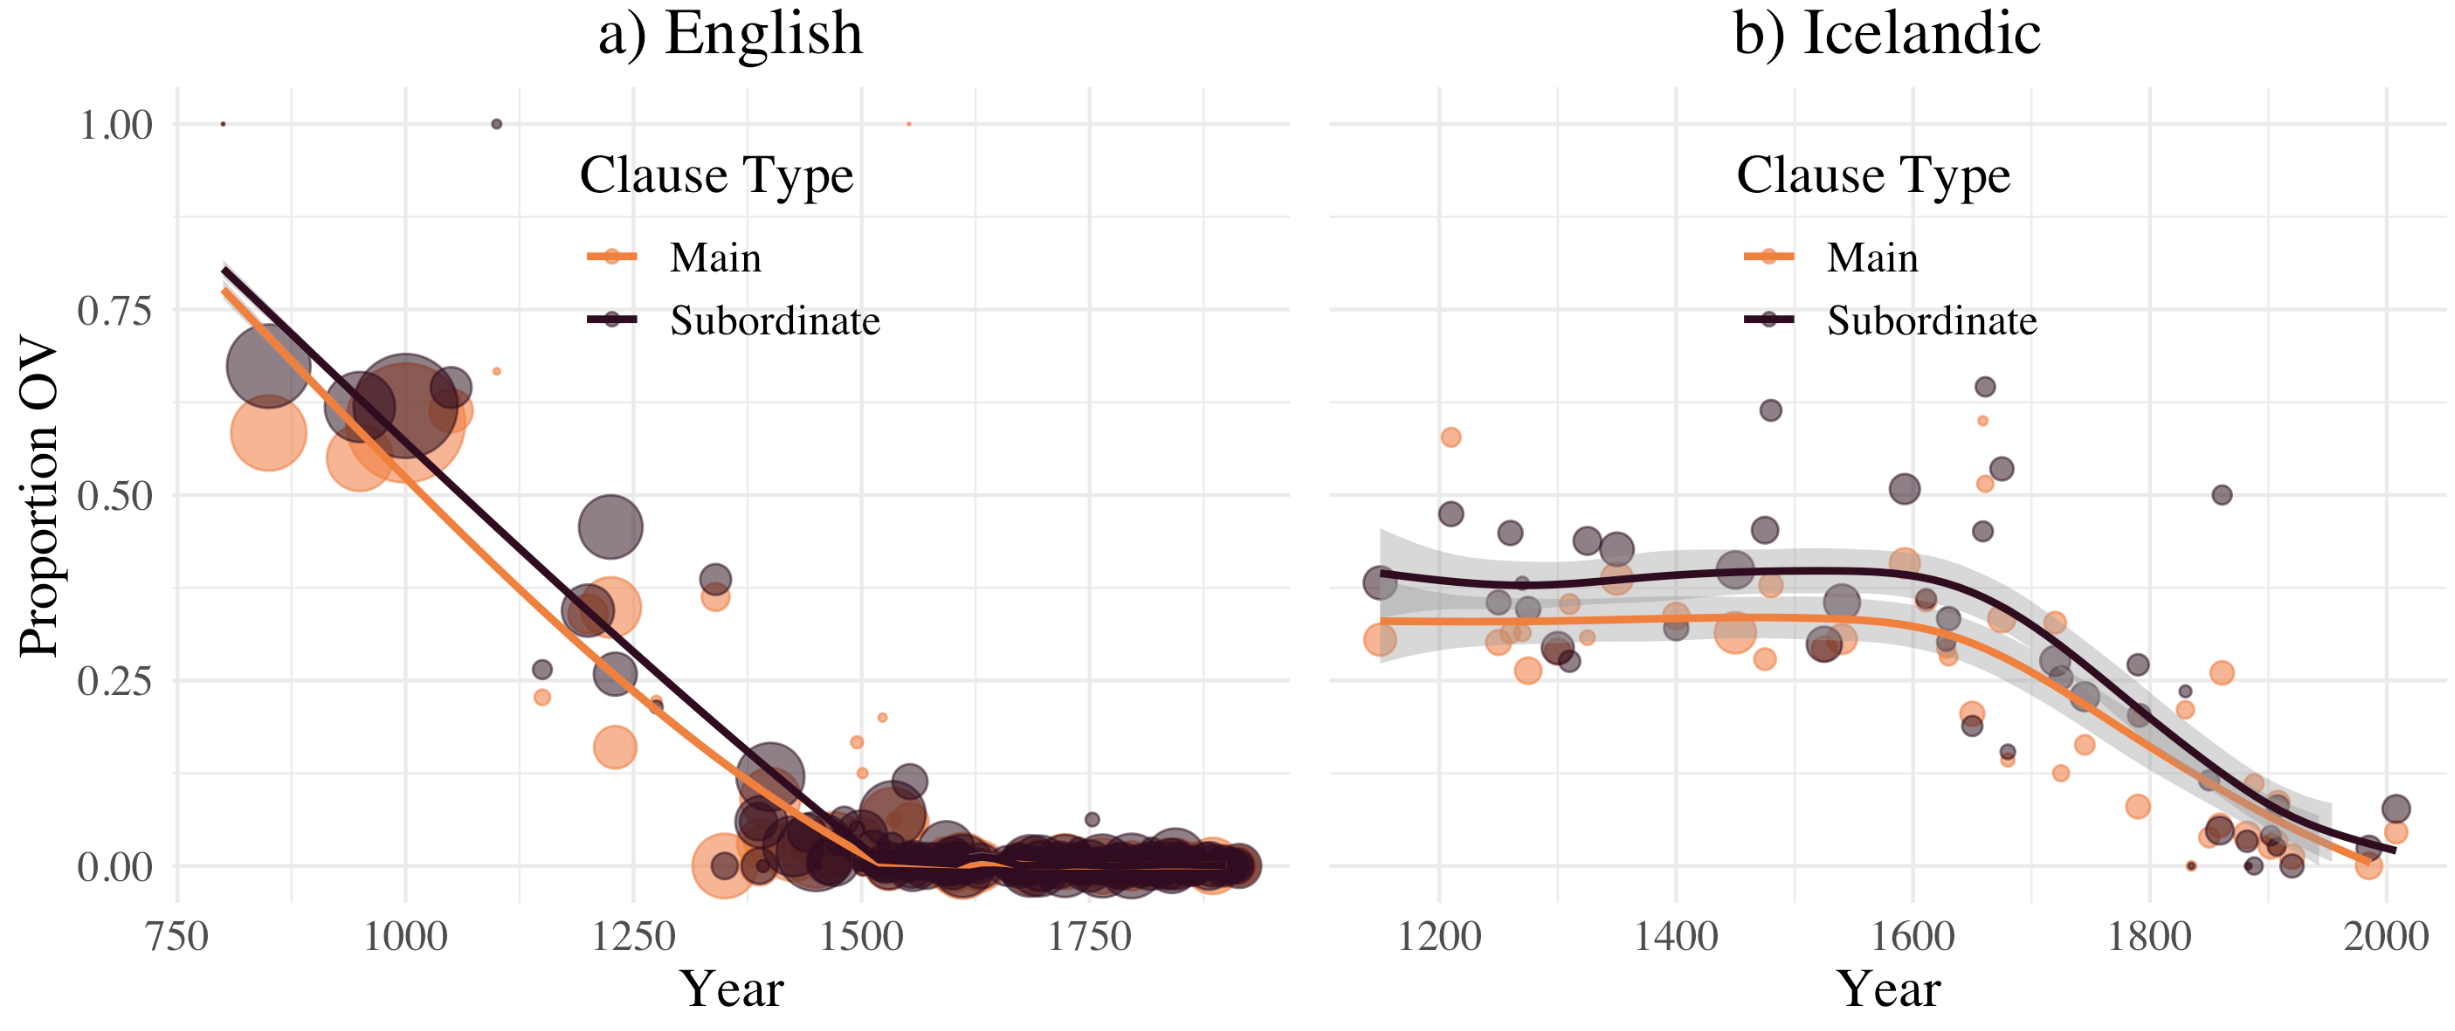
\includegraphics[width=1.04\textwidth]{FullClauseFig.png}
	\begin{itemize}
	\item Note the Constant Rate Effect \citep{kroch1989}, shown for English by \citet{pintzuktaylor2006}.
\end{itemize}	
\end{frame}

\begin{frame}{OV-to-VO and Information Theory} 
	
\begin{enumerate}
	\item Pronouns are closed-class and frequent, and so are low information content, (cf. \citealt{shannon1948}) in comparison with nominal DPs (e.g., \textsl{you} vs. \textsl{the politician}). For example, the average information content value for pronouns in the Penn Parsed Corpus of Modern British English (PPCMBE; \citealt{ppcmbe2}) is 11.7 bits.
	\item Nominal DP Objects are high information content in general, because any particular DP will be low probability. There are more common noun lexemes than any other part of speech, and so any given noun is lower probability by virtue of belonging to a very large set. The probability of a given noun \textit{combined with} a determiner and/or modifiers is necessarily lower than the probability of the noun alone. For example, the average information content for nouns in PPCMBE is 13.7 bits, and we can reasonably expect the average information content is much higher for nominal DPs, since they can be of arbitrary complexity.
	\item Verbs are mid-level in frequency and so also in information content: lower than nominal DPs, on average, but higher than pronouns. For example, the average information content for lexical verbs in the PPCMBE is 13.5 bits.
\end{enumerate}

Given these generalizations, we developed and tested the following hypotheses.

\begin{itemize}
	\item When Subject and Object are of the same type (i.e., both pronominal or both nominal), VO clause structure is statistically favored.
	\item Otherwise, OV clause structure is favored.
	\item These effects are orthogonal to the OV to VO change, but apply as constants throughout the course of the change.
\end{itemize}
\end{frame}


\begin{frame}
	
	\begin{center}
	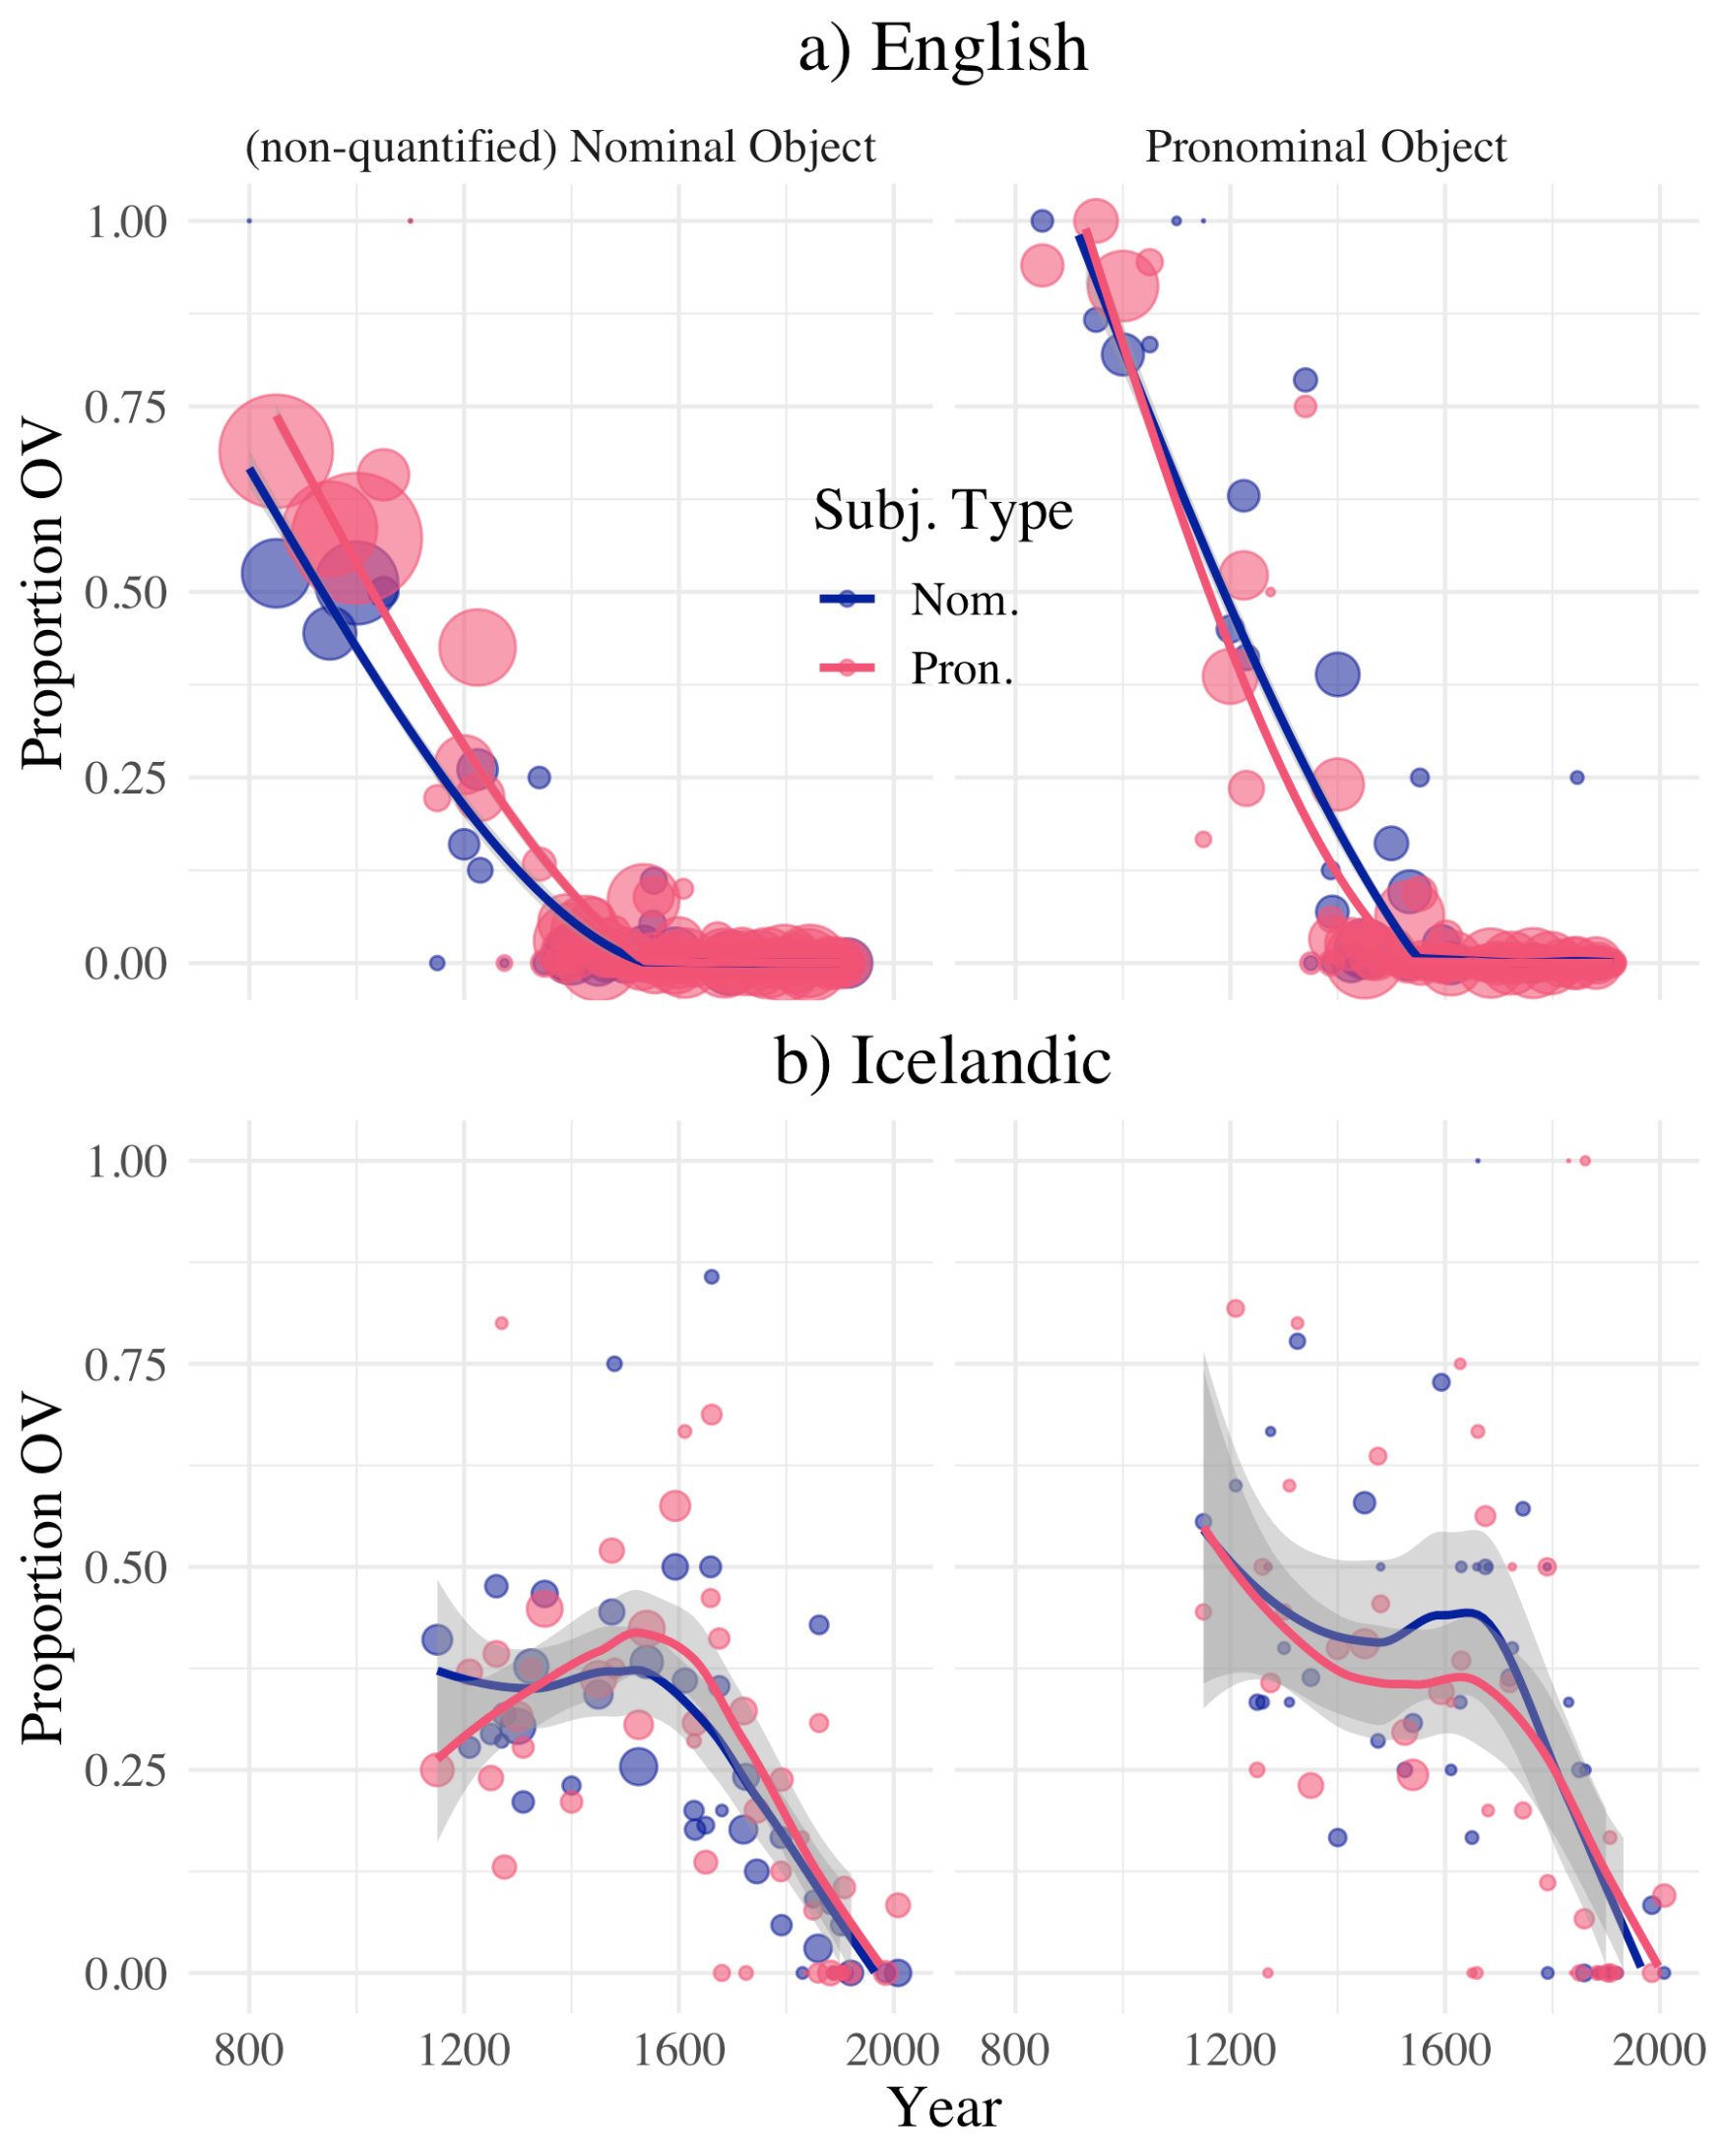
\includegraphics[scale = 0.5]{Fig3-4.png}
	\end{center}
\end{frame}



\section{Study 2: OV and VO variation in historical Icelandic}


\begin{frame}{DORM} 


XXX
lemmas

\end{frame}


\begin{frame}%{OV, OV, and Information Uniformity in Icelandic} 
	
	
	\begin{center}
	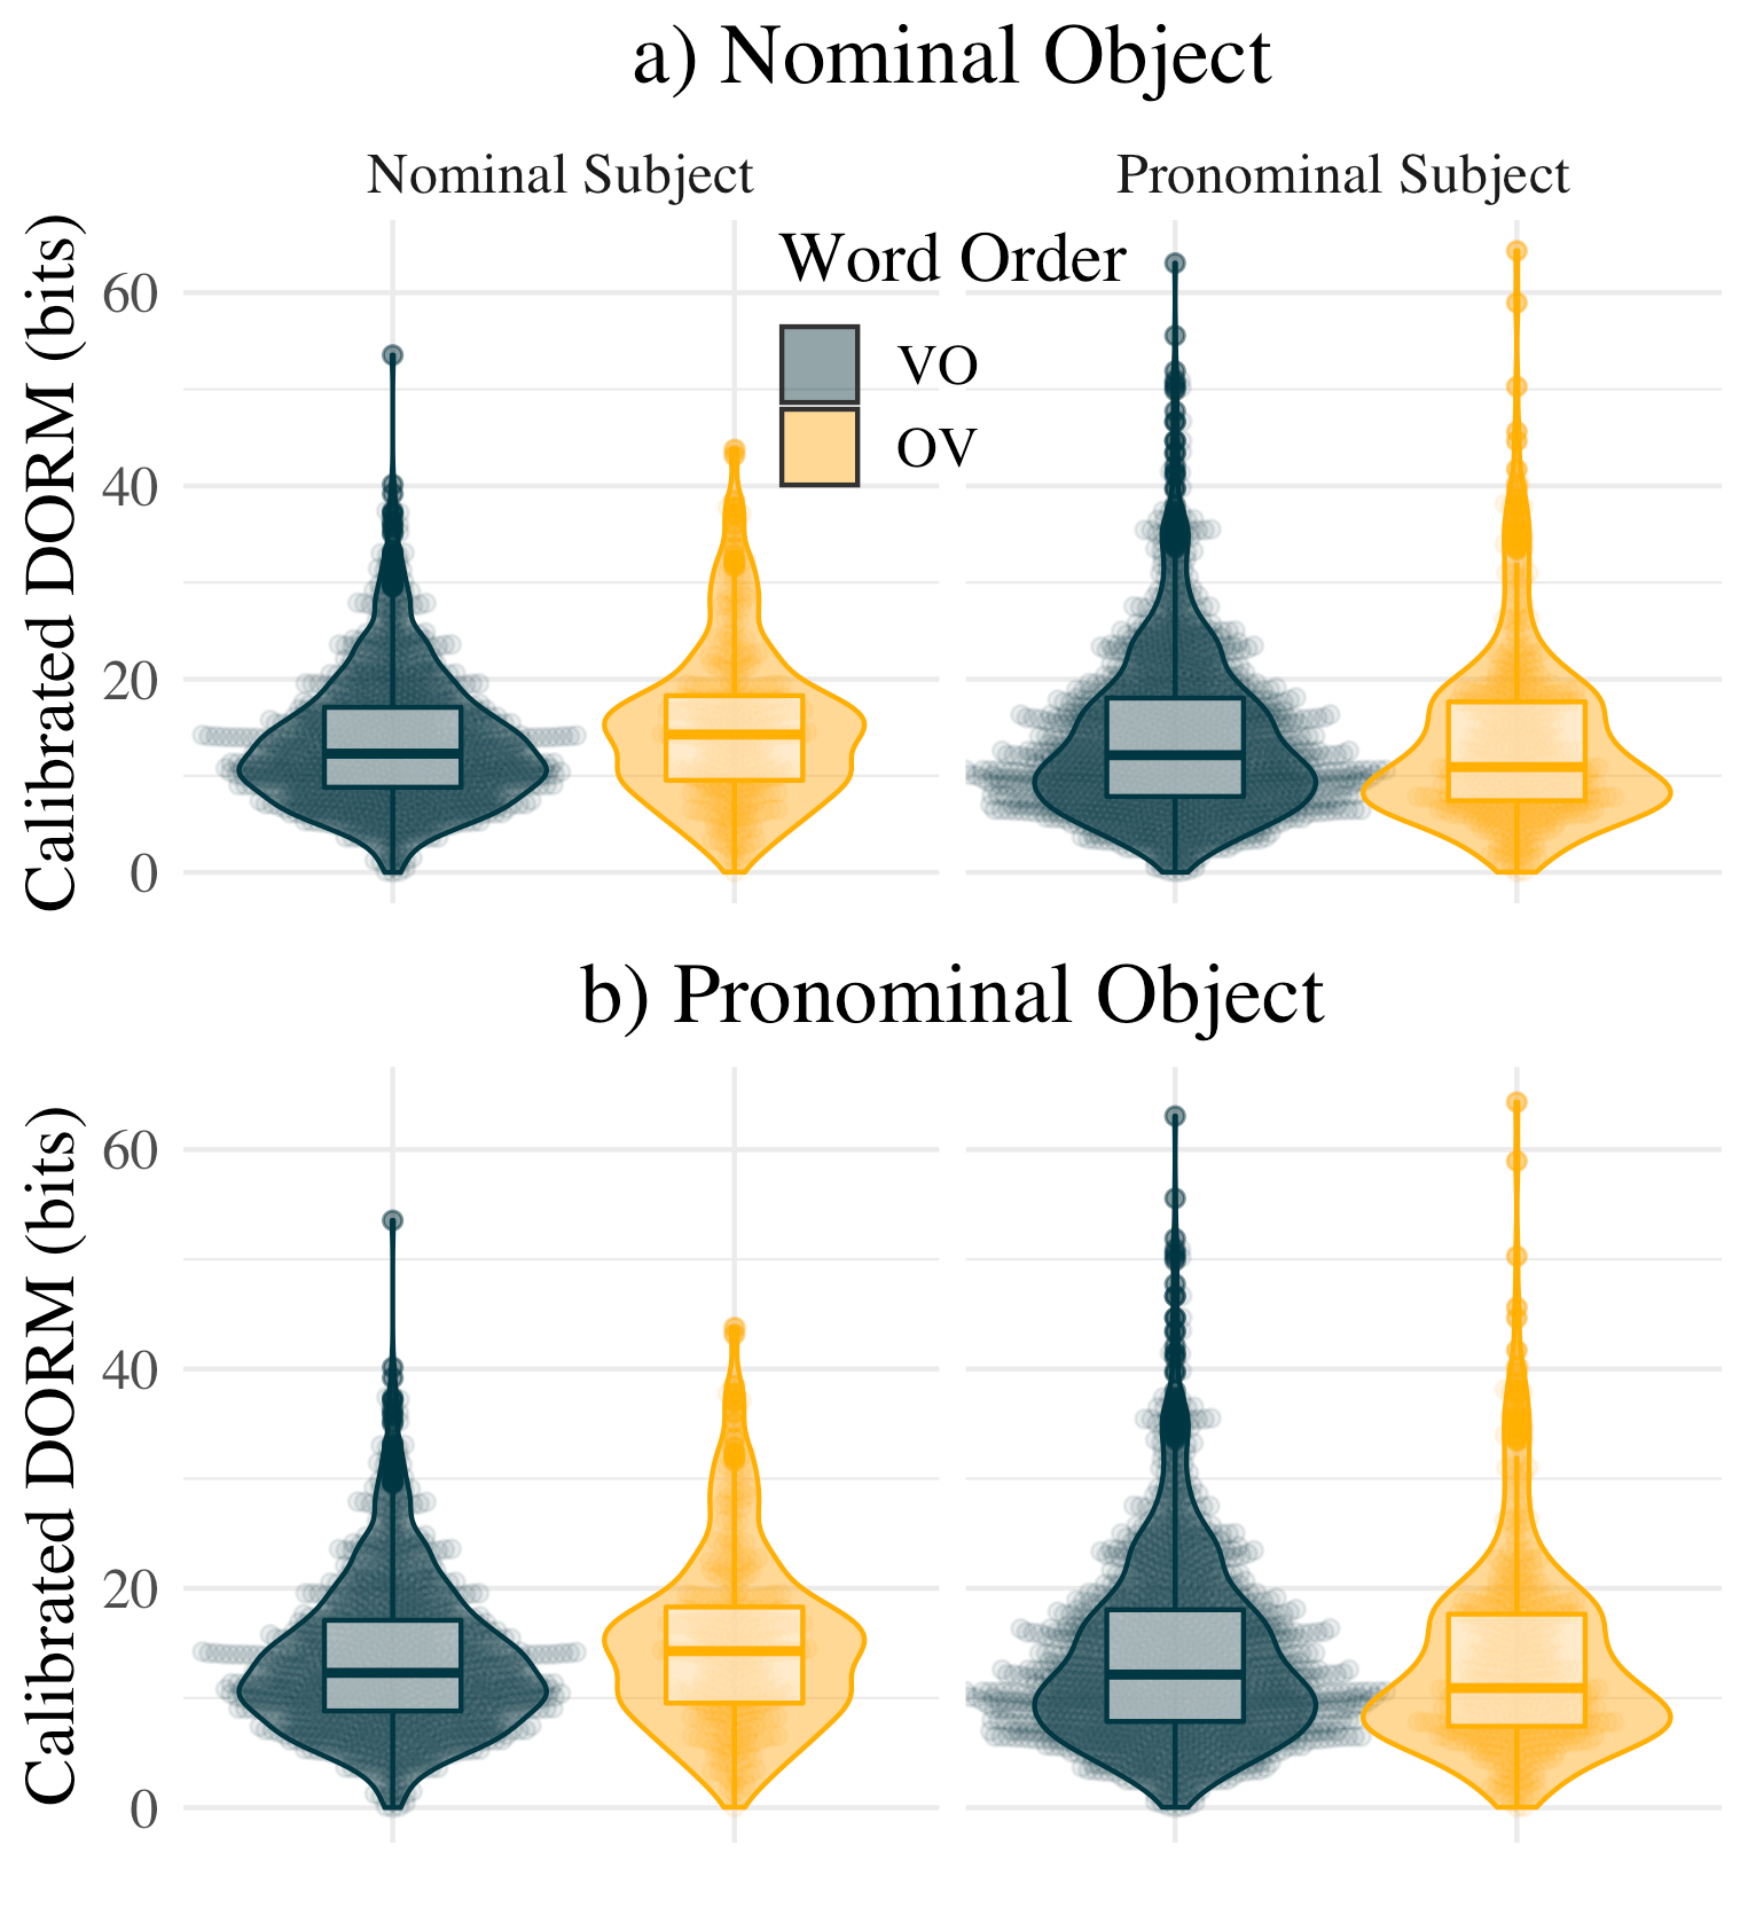
\includegraphics[scale = 0.5]{NewFigType3.png}
\end{center}
	
\end{frame}

\begin{frame}{What Doesn't Change, Doesn't Change} 
	
	
%	\begin{center}
		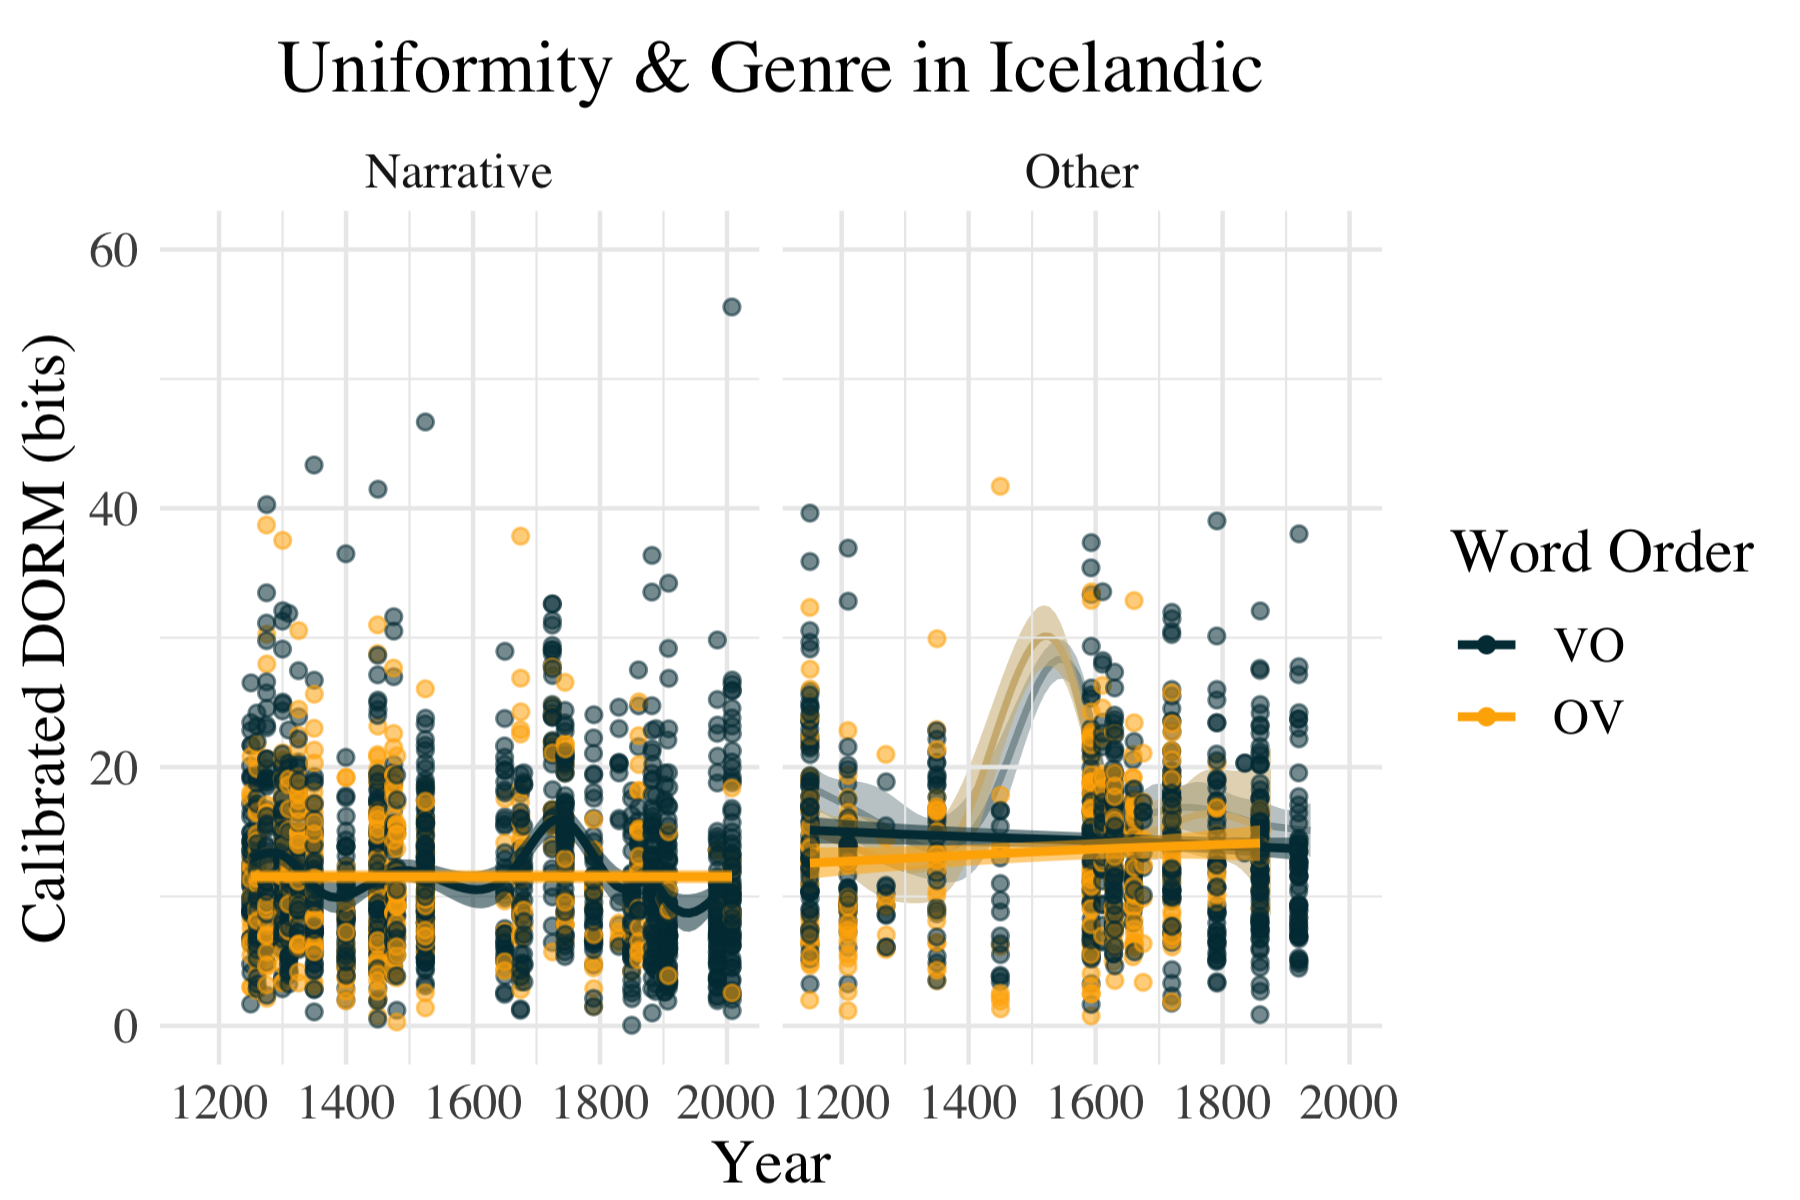
\includegraphics[scale = 0.2]{IcelandicGenreOutlierBehind.png}
%	\end{center}
	
\end{frame}

\begin{frame}{What Doesn't Change, Doesn't Change (Kroch, Labov, p.c.)} 
	
	
	\begin{center}
		variance XXX
	\end{center}
	
\end{frame}

\begin{frame}{Conclusions} 
	
	
	\begin{itemize}
		\item XXX
	\end{itemize}
	
\end{frame}


\begin{frame}{Future Directions} 
	
	
	\begin{itemize}
		\item XXX
	\end{itemize}
	
\end{frame}




\begin{frame}[allowframebreaks]
\frametitle{References}
\bibliographystyle{linquiry2}
\bibliography{joelrefs}
\end{frame}


\begin{frame}{Crash course} 
	\begin{itemize}
		\item The amount of information in a fair coin toss is 1 bit.
		\item The amount of information in an unfair coin toss with $$p = \frac{1}{3}, \frac{2}{3}$$ is less, even though less probable events have higher information content.
	\end{itemize}
	\begin{center}
		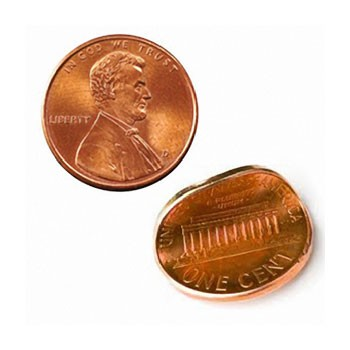
\includegraphics[scale=0.4]{bentcoin.jpg}
	\end{center}
\end{frame}


\end{document}